\documentclass[article,a4paper]{IEEEtran}
\usepackage[backend=biber]{biblatex}
\usepackage{graphicx}
\usepackage{lipsum}

\addbibresource{refs.bib}
\title{Powering the Future: Energy Harvesting and Intermittent Computing in IoT}
\author{
\IEEEauthorblockN{Anton Odén}\\
\IEEEauthorblockA{Dept. of Maths and Computer Science\\Karlstad University\\
651 88 KARLSTAD, Sweden}\\
anton.oden@outlook.com
}

\begin{document}

\maketitle

\begin{abstract}
Energy harvesting and intermittent computing are two paradigms that changes the design of IoT and embedded systems. By capturing ambient energy from solar, thermal, mechanical, biochemical and radio frequency sources, these technologies enable traditional battery-free operation. However, the inherent volatility of harvested energy necessitates new computing strategies. This articles delves into the challenges of maintaining execution state during power interruption and explores the frameworks Ratchet, Chinchilla and Alpaca. 
\end{abstract}

\tableofcontents
\subsection{Introduction}
The number of connected devices continues to grow and energy efficiency is an important consideration in computing and communication systems. Looking for autonomous, battery-free operation in IoT and embedded systems leads to adoption of energy harvesting, a technique that captures and converts ambient energy from sources such as solar radiation, thermal gradients, mechanical vibrations, biochemical reactions and radio frequency signals \cite{Energyharvest1}. This enables devices to operate in environments where battery replacements or wired connections are impractical. 
\newline\newline
However, energy harvesting presents challenges, particularly in maintaining reliable computation under unpredictable power availability. Unlike traditional computing which assumes continuous power, intermittent computing ensures progress despite sudden power interruptions by strategies such as checkpointing and task-based execution. Frameworks such as Ratchet, Chinchilla and Alpaca discussed in this article has been developed to enable efficient computing for small IoT devices running on unstable power supply.  
\newline\newline
This article explores energy harvesting, its impact on IoT devices and the role of intermittent computing frameworks in ensuring robust performance. Energy-harvesting could pave the way for a future where computing no longer depends on traditional batteries, reducing costs, improving longevity and expanding the reach of IoT. 
\begin{figure}
    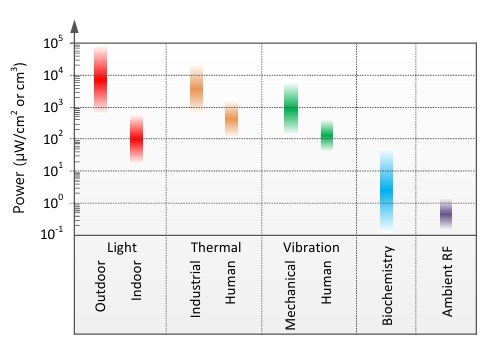
\includegraphics[width=\columnwidth]{EnergyHarvest1.png}
    \caption{ Different energy harvesting areas showing given energy from \cite{Energyharvest1} }
    \label{fig2_Energy_harvest}
\end{figure}
\subsection{Energy harvesting}
%\subsubsection{What is energy harvesting?}
Energy harvesting refers to the process of capturing and converting ambient energy from natural or artificial sources into usable electrical power. Common sources of harvested energy include solar radiation, thermal gradient, mechanical vibration, biochemical reactions and radio frequency \cite{Energyharvest1}. Unlike traditional power supplies, energy harvesting systems enable autonomous operation in environments where wired connection or battery replacements are impractical. This technique is increasingly vital for IoT devices and embedded systems with batter-free computing where maintaining continuous power supply is challenging or that cutting the cost of battery is the next step in making IoT devices even more cheap. Instead of traditional batteries, capacitors can be used instead that can hold energy for a shorter duration of time but are better adapt for long life. Rechargeable batteries has limited number of recharge cycles on the order of 1000, meaning that rechargeable batteries needs to be replaced, which could be a costly action dependent on location of IoT devices and the staggering number of devices that the future could have. Supercapacitors are able to be recharged over a million of time and are able to let out energy quicker than a battery if that is something that is necessary for the IoT device. The circuit is also to be deemed more simple according to \cite{Energyharvest1}. 
\newline\newline 
%\subsubsection{RF energy harvesting and the WISP project}
One intriguing technology in energy harvesting is RF (radio frequency) energy harvesting \cite{RF_energy_harvest}, which can utilize electromagnetic waves from sources such as cell towers and WiFi signals to generate power. As RF communication is deemed to increase in an IoT world the amount of energy possible to harvest from RF is deemed to increase. A study made in four American cities in 2014 measured power density to be less than $1\mu W\/{cm}^2$ in 90\% of measured area. Another study from Stockholm inner-city measured over 1mW on some frequencies as can be seen in figure \ref{fig1_energy_sthlm}. A succeeding master study from 2024 instead lowered these measurements to just peak at 1mW on 865-868mHz band. The master study states that ~3mW is required to harvest energy from radio waves so it's problematic to just rely on passive RF signals still. However if the application is known to harvest energy it is possible to position the application/device in a location that is known to have better signals (close to transmitting antennas) \cite{Master_ambient_rf}.
\newline\newline
The WISP Wireless identification and sensing platform project exemplifies this approach \cite{WISPproject}, demonstrating how RF energy can support battery-free computation and sensing. WISP operates using passive RFID technology, converting radio waves into energy enough for tasks like data processing and sensor driven applications. This enables devices to function in environments with consistent RF energy exposure, pawing the way for battery-free IoT solutions.
\begin{figure}
    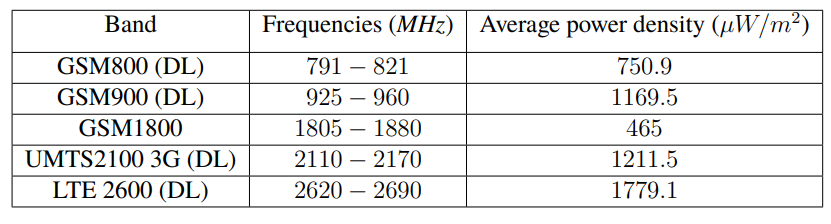
\includegraphics[width=\columnwidth]{Ambientradiofrequency.png}
    \caption{ Table showing power density on some picked frequencies in inner Stockholm from \cite{RF_radiation_sthlm} }
    \label{fig1_energy_sthlm}
\end{figure}
\newline\newline
%\subsubsection{Challenges in energy-harvesting}
Despite advantages of IoT devices able to compute and communicate without traditional battery. Energy harvesting does has a challenge with ambient energy fluctuation leading to unpredictable power levels. This leads to systems required to adopt intermittent computing strategies such as e.g. Alpaca, Ratchet and Chinchilla further discussed in this article. However if the IoT devices dependent on energy harvesting is good enough for the overall system, if it is able to compute and communicate only during times when energy harvesting is possible, traditional batteries can be replaced by capacitors that creates cheaper and less bulky products able to have very long life.  
\subsection{Understanding intermittent computing}
Intermittent computing is designed for systems that experience frequent power interruptions, often seen in energy-harvesting devices. Unlike traditional computing, which assumes continuous power availability, intermittent systems must execute tasks in small steps, ensuring progress even during power failures. 
%\subsubsection{Why traditional computing fails under unstable power?}
\newline\newline
Counter to traditional computing that could be considered to be continuous. Intermitted computing is able to handle planned or unplanned breaks in computation. The processor in itself does not have a problem with power breaks but the memory used in computation to write and read data is more or less stored in volatile memory, for example RAM, Cache, CPU registers. Meaning that it doesn't uphold data during power loss. Memory that does keep data during power loss is non-volatile and could be for example FRAM, Flash, EEPROM. Traditional computing then fails under unstable power as memory used by computation is lost and there is no checkpoints to know what state the computation and memory was in close to power loss so the computation results can't be trusted to be correct if it wouldn't restart from beginning. Energy harvesting dependent systems has to operate intermittent as the energy harvested can't assumed to be constant, but instead is loosing power frequently and unexpectedly. 
\newline\newline
%\subsubsection{Strategies for reliable computation with energy harvesting}
Since power availability differs in energy-harvesting systems, computing strategies must adapt. Some key approaches include, \textbf{checkpointing} that regularly saves system state so computation can resume at last checkpoint (e.g. Chinchilla and Ratchet). \textbf{Task-based execution} where program is broken into small self-contained tasks that restarts after power loss (Alpaca). \textbf{Non-volatile memory} usage, storing of execution data in FRAM or Flash memory to preserve progress. 

\subsection{Frameworks for intermittent computing}
Intermittent computing requires specialized compilation techniques to ensure programs can function despite unpredictable power failures. Unlike traditional compilation, which assumes continuous execution, intermittent computing frameworks modify code execution behavior so systems can resume operations seamlessly after a power outage. These frameworks aim to prevent data loss when power fails, enable efficient recovery without manual intervention and optimize execution for low-power environments. 
\newline\newline
Since energy-harvesting devices operate with instable power, normal software execution fails because variables, loop states and memory data disappear when power is lost. Specialized compilation frameworks enhance program by automatically adding checkpoints to preserve state (Ratchet) or adjusts checkpoint frequency dynamically based on power availability (Chinchilla). Iterated computation statements could in compilation be flagged as non-idempotent and temporary variables is added by compilers (Alpaca). 
\newline
\subsubsection{\textbf{Ratchet}}
Ratchet provides compiler-based automatic checkpointing which makes it possible to use without hardware support \cite{Ratchet}, meaning standard microcontrollers could be used. Ratchet inserts checkpoints in compilation without requiring programmer to modify code manually. The checkpoints creates idempotent sections of the code where write and read (WAR)-instructions are separated to avoid problem that could arise when program gets interrupted in the middle of a section. This problem is illustrated in \ref{fig3_WAR_problem} showing memory writes affects computation on restart. 
\newline\newline
Ratchet transform execution state into safe recoverable snapshots, ensuring program resume smoothly after power loss. It ensures redundancy is minimized to prevent unnecessary recomputation. The code for Ratchet is open sourced since 2016 via \cite{Ratchetsrc}.
\begin{figure}
    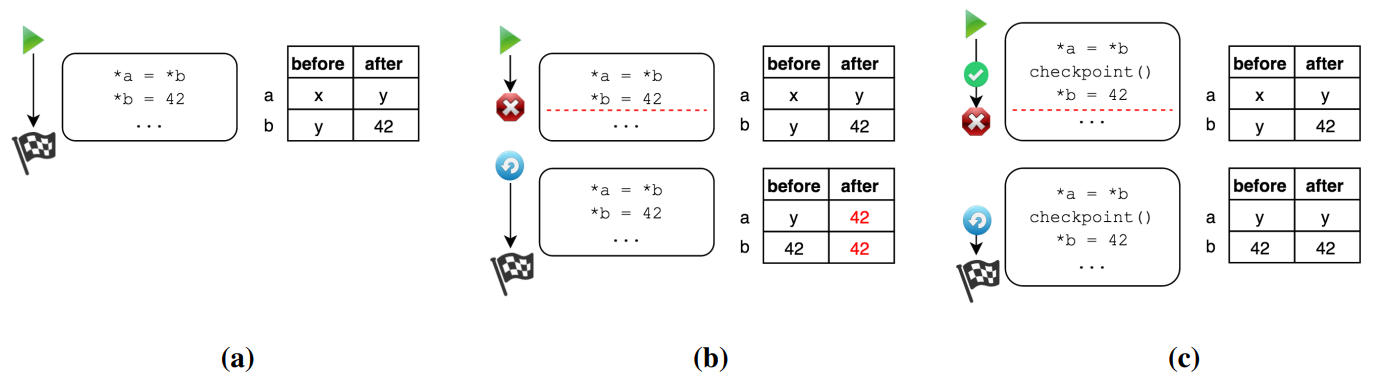
\includegraphics[width=\columnwidth]{WAR-problem.png}
    \caption{ Basic example illustrating difficulties with using non-volatile main memory on intermittent powered computers from \cite{Ratchet} }
    \label{fig3_WAR_problem}
\end{figure}
\newline
\subsubsection{\textbf{Alpaca}}
In Alpaca more work is on the programmer to divide programs into tasks and add gotos (transition\_to) at the end of each task \cite{Alpaca}. The programmer needs to be aware of the amount of energy that is possible at a minimum to compute with so a task is not to large and thereby not able to finish. As the program overhead is handed to the programmer there is more room for designing efficient code adapted to the device environment which could differs largely between devices, at the same time it is possible to create very inefficient code as it depends on the programmers skill level. Overhead is limited to every individual task write to non volatile memory at the end of a task. Second feature-leg for Alpaca is privatization that guarantees that volatile or non-volatile memory access by a task remains consistent, regardless of power failure. 
\newline\newline
Alpaca divides data into task-shared and task-local data. Task-shared variables are in the global scope and are allocated in a non-volatile memory and once a task writes a value to a task-shared variable, that same task or another task may later read the value. In Alpaca the compiler backtracks write and reads to all task-shared variables to decide if tasks needs to privatize usage of variables, meaning that a local variable is created in tasks and in the end of task a commit to task-shared variable is done before transitioning to next task. Task-local variables are scoped only to a single task and must be initialized by that task and are allocated in volatile memory.
\newline\newline
Committing of data from volatile to non-volatile memory is done in two phases and flags are changed to signal what phase the task was in when rebooting after power interruption. First pre-commit creates a table in non volatile memory with all values to be changed in the task-shared scope. If interrupted during this phase the whole task needs to be computed from beginning. After pre-commits done, commit\_ready is set to \texttt{true} and Alpaca runtime during reboot knows to jump to commit-phase directly. In commit-phase task-shared variables are changed in non-volatile memory. When commit-phase is done commit\_ready flag i removed and end-index is set to zero. So that the Alpaca runtime knows that transition to next task is the only step left to do on reboot. To support privatization the programmer needs to specify task-shared variables for the Alpaca compiler to guarantee consistency of data.
\newline\newline
Alpaca was developed by Kian Maeng, Alexei Colin and Brandon Lucia at Carnegie Mellon University in USA with presentation of its work 2017. The source code for runtime environment can be found on github \cite{Alpacasrc}. It has been developed in different versions as the text in \cite{Alpaca} presents Alpaca-redo, Alpaca-undo and Alpaca-VM that uses the same approach of dividing program into tasks but handles the memory in different fashion. The privatization of data and commit-phases prior described follows the Alpaca-redo runtime system. Alpaca-undo does instead work with variables in task-shared scope directly but does keep a list of back-up variables that writes over changes done to task-shared variables in case of power failure. This makes Alpaca-undo more efficient than Alpaca-redo for systems that are assumed to not have a task power fail more often than succeeding computation.  
\begin{figure}
    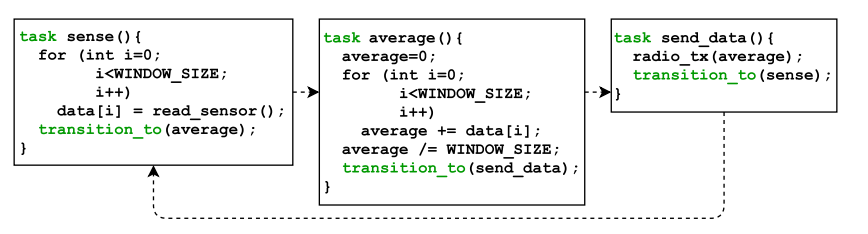
\includegraphics[width=\columnwidth]{Alpacatasksexample.png}
    \caption{ Example application written i Alpaca from \cite{Alpaca} }
    \label{fig4_Alpaca_tasks}
\end{figure}
\newline
\subsubsection{\textbf{Chinchilla}}
Chinchilla introduces dynamic checkpointing that adjust checkpoint frequency based on available energy to maximize efficiency \cite{Chinchilla}. Chinchilla does include a lot of checkpoints from compilation in the code but dynamically chooses to activate them during runtime. This reduces overhead by choosing only necessary checkpoints instead of static checkpointing as in Ratchet. Chinchilla uses runtime monitoring to determine when a checkpoint should be taken. It's algorithm considers current power fluctuation, past energy trends in previous cycles and computation critical sections when deciding which frequency to activate checkpoints at. 
\newline\newline
Chinchilla can be seen as influenced by the work of Ratchet but enhancing the idea of checkpoints from Ratchet and adapt it more for low-power IoT devices. It was developed by some of the same persons building Alpaca at Carnegie Mellon University. The source code can be found at \cite{Chinchillasrc} and the article and code was published 2018 following their work on Alpaca by a year.  

\subsection{Discussion and future directions}
I expect energy harvesting to keep increasing. Gardening and other fields is already today flushed by cheap solar radiation harvesting accessories but that lacks the IoT capabilities. Super capacitors still can hold it's energy over the night at an accepting rate. According to \cite{RF_energy_harvest} loosing 50\% of energy within a month a few cloudy days would still keep low power sensors powered depending on energy required for compute and collecting of data. 
\newline\newline
RF energy recharging is something already used in for example RFID tags that gets powered by RFID reader enough to be able to send information to validate identification. The automation of more application within society does benefit from close range recharging of batteries as connecting of cables for charging is something hard to automate. The article \cite{Master_ambient_rf} discuss the already available sensor product used in dairy industry, where cows has a neckless sending data about cows behavior and psychical health. Today these applications uses batteries that needs to be replaces but with RF stations being located at for example milking stations or food benches the neckless could be recharged at a daily basis. Reducing costs of battery replacement. 
\newline\newline
Another example I stubbled upon visiting a friend was a kitchen scale being driven by the user spinning a wheel to give it temporary energy\cite{Kitchen_scale}. There are probably tons of these products where the sensor or actuator is only needed a short duration when the user is present and harvesting small vibrations or kinetic energy from the user is a price the user is willing to pay instead of the risk of having to trash the product then battery needs replacement and the battery is so product specific that it is not possible to buy anymore. 
\begin{figure}
    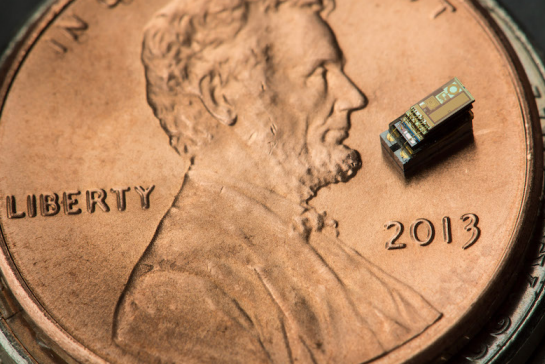
\includegraphics[width=\columnwidth]{Smartdust.png}
    \caption{ Smart dust developed by University of Michigan, sitting of a American penny from \cite{RF_energy_harvest} }
    \label{fig5_smart_dust}
\end{figure}
\begin{figure}
    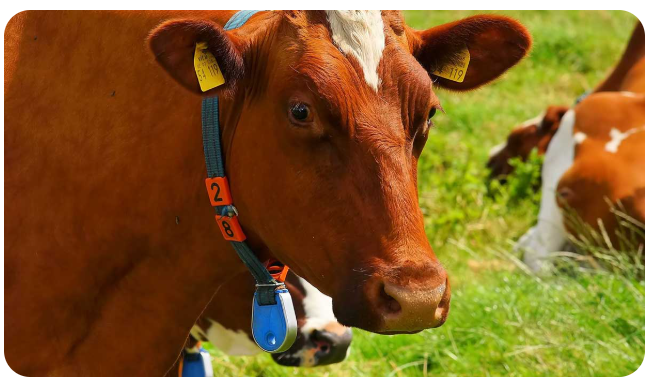
\includegraphics[width=\columnwidth]{Cowsensors.png}
    \caption{ Sensors attached to cows developed by Prevas from \cite{RF_energy_harvest} }
    \label{fig6_cow_sensor}
\end{figure}
\subsection{Conclusion}
In this article we have discussed intermittent computing, energy harvesting, with a particular focus on how ambient RF energy can power IoT sensors in battery-free environments. We examined how challenge of unstable power, which is common in energy-harvesting systems, necessitates new strategies in software design. 

Intermittent computing adds a layer of consideration for the programmer and device designer. To address the critical challenge of preserving program state during unexpected power interruptions, we highlighted three different frameworks: Ratchet, Chinchilla and Alpaca. 
\newline\newline
As IoT continuous to expand. Energy harvesting and intermittent computing is set to play an increasingly critical role. By enabling devices to operate automously without traditional batteries, these techniques can reduce costs both in production but also in battery change maintaining.  
\printbibliography

\end{document}